\documentclass{article}%
\usepackage[T1]{fontenc}%
\usepackage[utf8]{inputenc}%
\usepackage{lmodern}%
\usepackage{textcomp}%
\usepackage{lastpage}%
\usepackage[head=40pt,margin=0.5in,bottom=0.6in]{geometry}%
\usepackage{graphicx}%
%
\title{\textbf{Docentes de Guárico protestan por mejoras salariales}}%
\author{EL NACIONAL WEB}%
\date{03/12/2018}%
%
\begin{document}%
\normalsize%
\maketitle%
\textbf{URL: }%
http://www.el{-}nacional.com/noticias/protestas/docentes{-}guarico{-}protestan{-}por{-}mejoras{-}salariales\_261928\newline%
%
\textbf{Periodico: }%
EN, %
ID: %
261928, %
Seccion: %
Protestas\newline%
%
\textbf{Palabras Claves: }%
Crisis económica, Protestas, Sociedad\newline%
%
\textbf{Derecho: }%
2.3, %
Otros Derechos: %
, %
Sub Derechos: %
2.3.4\newline%
%
\textbf{EP: }%
SI\newline%
\newline%
%
\textbf{\textit{Los profesionales de la educación se reunieron en San Juan de los Morros para reclamar por mejores condiciones laborales~}}%
\newline%
\newline%
%
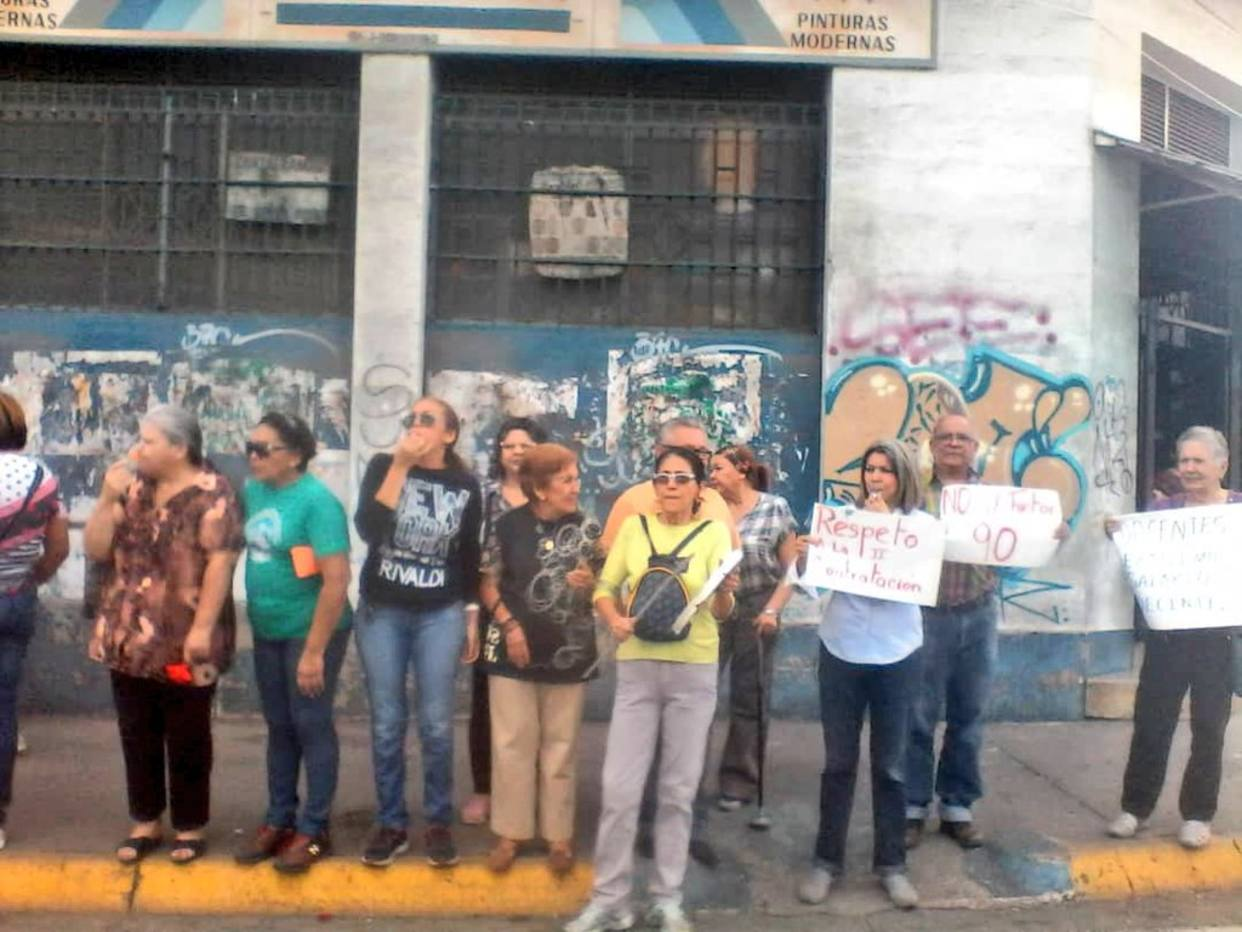
\includegraphics[width=300px]{55.jpg}%
\newline%
%
El gremio de docentes del estado Guárico inició una protesta durante la mañana de este martes en la Zona Educativa, de San Juan de los Morros, para exigir mejores condiciones laborales.%
\newline%
%
Los profesionales de la educación reclamaron con pancartas por salarios dignos y tabuladores que “dignifiquen” la carrera de los docentes.%
\newline%
%
La información fue compartida mediante Twitter por Radio Fe y Alegría.%
\newline%
%
\end{document}